% !TeX program = xelatex
\documentclass[a4paper,10pt]{article}

% ============================================================================
% សន្លឹកកិច្ចការសិស្ស ស-ខ្មៅ (Student Guided-Inquiry Worksheet - Grade 8 ALG58)
% បរិបទ៖ ថ្នាក់រៀនគ្មានស្លាយ LCD – ៤.២ (ត) បំពេញការេ បំបែកតួកណ្ដាល និងការផ្ដុំតួ (២ ទំព័រ A4)
% ============================================================================
\usepackage[a4paper, left=0.90cm, right=0.90cm, top=0.75cm, bottom=0.85cm, footskip=0.45cm]{geometry}
\usepackage{amsmath, amssymb}
\usepackage{unicode-math}
\usepackage{fontspec}
\usepackage{array, colortbl}
\usepackage[table]{xcolor}
\usepackage{enumitem}
\usepackage{pifont}
\usepackage{fancyhdr}
\usepackage{lastpage}
\usepackage{tikz}
\usepackage[most]{tcolorbox}
\usetikzlibrary{calc, arrows.meta, positioning, babel}

\makeatletter
\let\@expl@@@mark@update@singlecol@structures@@\relax
\makeatother

\providecommand{\NGSFindFonts}{%
  \IfFileExists{C:/Windows/Fonts/cambria.ttc}{%
    \def\NGSSysPath{C:/Windows/Fonts/}%
    \def\NGSUserPath{C:/Users/KIT/AppData/Local/Microsoft/Windows/Fonts/}%
  }{%
    \IfFileExists{./fonts/KhmerOSsiemreap.ttf}{\def\NGSSysPath{./fonts/}\def\NGSUserPath{./fonts/}}{%
    \IfFileExists{../fonts/KhmerOSsiemreap.ttf}{\def\NGSSysPath{../fonts/}\def\NGSUserPath{../fonts/}}{%
    \IfFileExists{../../fonts/KhmerOSsiemreap.ttf}{\def\NGSSysPath{../../fonts/}\def\NGSUserPath{../../fonts/}}{%
    \IfFileExists{../../../fonts/KhmerOSsiemreap.ttf}{\def\NGSSysPath{../../../fonts/}\def\NGSUserPath{../../../fonts/}}{%
    \IfFileExists{../../../../fonts/KhmerOSsiemreap.ttf}{\def\NGSSysPath{../../../../fonts/}\def\NGSUserPath{../../../../fonts/}}{%
    \IfFileExists{../../../../../fonts/KhmerOSsiemreap.ttf}{\def\NGSSysPath{../../../../../fonts/}\def\NGSUserPath{../../../../../fonts/}}{%
    \IfFileExists{../../../../../../fonts/KhmerOSsiemreap.ttf}{\def\NGSSysPath{../../../../../../fonts/}\def\NGSUserPath{../../../../../../fonts/}}{%
      \def\NGSSysPath{../../../../../../../fonts/}\def\NGSUserPath{../../../../../../../fonts/}%
    }}}}}}}%
  }%
}
\NGSFindFonts

\setmathfont[Path={\NGSSysPath}, FontIndex=1, Scale=1.02]{cambria.ttc}
\defaultfontfeatures{Ligatures=TeX}

\setmainfont[
  Path={\NGSUserPath},
  Extension=.ttf,
  Script=Khmer,
  BoldFont={KhmerOSsiemreap},
  BoldFeatures={FakeBold=1.8},
  ItalicFont={KhmerOSsiemreap},
  ItalicFeatures={FakeSlant=0.25},
  BoldItalicFont={KhmerOSsiemreap},
  BoldItalicFeatures={FakeBold=1.8, FakeSlant=0.25}
]{KhmerOSsiemreap}

\newfontfamily\muol[Path={\NGSUserPath}, Extension=.ttf, Script=Khmer]{KhmerOSmuollight}
\newfontfamily\TimesEn[Path={\NGSSysPath}, Extension=.ttf, BoldFont={timesbd}, ItalicFont={timesi}, BoldItalicFont={timesbi}]{times}

\XeTeXlinebreaklocale "km"
\XeTeXlinebreakskip = 0pt plus 1pt minus 0.1pt

\definecolor{panelgray}{gray}{0.94}
\definecolor{headgray}{gray}{0.86}

\pagestyle{fancy}
\fancyhf{}
\renewcommand{\headrulewidth}{0pt}
\fancyfoot[L]{\fontsize{8pt}{10pt}\selectfont អនុវិទ្យាល័យព្រះក្រសាំង \en{|} គណិតវិទ្យា ថ្នាក់ទី៨ \en{|} មេរៀនទី៥ (៤.២ត បំពេញការេ បំបែកតួកណ្ដាល និងការផ្ដុំតួ)}
\fancyfoot[R]{\fontsize{8.2pt}{10pt}\selectfont ទំព័រ \en{\thepage\ / \pageref{LastPage}}}

\setlength{\parindent}{0pt}
\setlength{\parskip}{0pt}
\setlength{\tabcolsep}{4pt}

\newcommand{\en}[1]{{\TimesEn #1}}
\newcommand{\enbf}[1]{{\TimesEn\textbf{#1}}}
\newcommand{\unit}[1]{\,\text{\en{#1}}}
\newcommand{\cnum}[1]{{\fontsize{10pt}{12pt}\selectfont\ding{\numexpr171+#1\relax}}}
\newcommand{\chk}{\tikz[baseline=-0.15ex]\draw[black, line width=0.8pt] (0,0) rectangle (0.25cm,0.25cm);}
\newcommand{\dotline}[1]{\makebox[#1]{\dotfill}}

\newcolumntype{L}[1]{>{\raggedright\arraybackslash}p{#1}}
\newcolumntype{C}[1]{>{\centering\arraybackslash}p{#1}}

\newcommand{\secbar}[2]{%
  \vspace{5pt}
  \noindent\colorbox{headgray}{\parbox{\dimexpr\linewidth-2\fboxsep\relax}{%
    \vspace{1.8pt}{\muol\fontsize{9.5pt}{13.5pt}\selectfont #1}\hfill{\fontsize{8.5pt}{12pt}\selectfont\textbf{#2}}\vspace{1.8pt}%
  }}\par\vspace{5pt}
}

\begin{document}
\fontsize{9.5pt}{14.2pt}\selectfont

% ============================================================================
% ទំព័រទី១៖ ក្បាលសន្លឹកកិច្ចការ + E1 + E2 + E3
% ============================================================================
\begin{tcolorbox}[enhanced, sharp corners, colback=white, colframe=black, boxrule=1.0pt, top=4pt, bottom=4pt, left=6pt, right=6pt]
  \begin{center}
    {\muol\fontsize{10.5pt}{15pt}\selectfont សន្លឹកកិច្ចការសិស្ស — មេរៀនទី៥៖ កន្សោមពីជគណិត \enbf{(}៤.២ត របៀបផ្សេងៗនៃការដាក់ជាផលគុណកត្តា\enbf{)}}\\[2pt]
    {\footnotesize សៀវភៅសិក្សាគោលថ្នាក់ទី៨ ទំព័រ ៧១--៧៤ \en{|} បំពេញការេ បំបែកតួកណ្ដាល ($ac$) និងការផ្ដុំតួ ២+២ ឬ ៣+១ (គ្មានស្លាយ \en{LCD})}
  \end{center}
  \vspace{2pt}
  \hrule height 0.5pt
  \vspace{4pt}
  ឈ្មោះសិស្ស៖ \dotline{5.3cm} ថ្នាក់៖ \dotline{2.0cm} ដៃគូទី៖ \dotline{2.0cm} កាលបរិច្ឆេទ៖ \dotline{3.3cm}
\end{tcolorbox}

% -------------------- ផ្នែកទី១៖ E1 ENGAGE --------------------
\secbar{ផ្នែកទី១ ៖ បេសកកម្មភ្ជាប់បញ្ហា \enbf{(E1 — Engage)} — ត្រីធាដែលមិនមែនជាការេទ្វេធា!}{\en{3} នាទី (ទស្សន៍ទាយមុនរៀន)}

\begin{tcolorbox}[enhanced, sharp corners, colback=panelgray, colframe=black, boxrule=0.8pt, top=3.5pt, bottom=3.5pt, left=6pt, right=6pt]
  \begin{minipage}[c]{12.2cm}
    ១) យើងដឹងថា $x^2 - 2x + 1 = (\dotline{1.8cm})^2$ ។ ចុះ $A = x^2 - 2x - 8$ (ទំ.៧១) តួចុងគឺ $-8$ មិនមែនការេទេ!\\[2pt]
    ២) \textbf{ទស្សន៍ទាយមុនរៀន៖} បើថែម-ថយ $1$ លើ $x^2 - 2x - 8 = (x^2 - 2x + 1) - 1 - 8$ តើវាស្មើកន្សោមណា?\\[1.5pt]
    \hspace*{0.3cm}\chk\ $(x - 1)^2 - 7$ \qquad\qquad
    \chk\ $(x - 1)^2 - 3^2$ \qquad\qquad
    \chk\ $(x - 4)^2$
  \end{minipage}\hfill
  \begin{minipage}[c]{6.0cm}
    \centering
    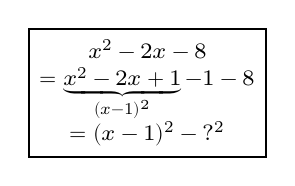
\begin{tikzpicture}
      \node[draw=black, line width=0.8pt, fill=white, inner sep=4pt, font=\footnotesize, align=center] {
        $x^2 - 2x - 8$\\
        $= \underbrace{x^2 - 2x + 1}_{(x-1)^2} - 1 - 8$\\
        $= (x-1)^2 - \mathbf{?}^2$
      };
    \end{tikzpicture}
  \end{minipage}
\end{tcolorbox}

% -------------------- ផ្នែកទី២៖ E2 EXPLORE --------------------
\secbar{ផ្នែកទី២ ៖ រុករកវិធីបំពេញការេ បំបែកតួកណ្ដាល និងការផ្ដុំតួ \enbf{(E2 — Explore)}}{\en{11} នាទី (ពិភាក្សាដៃគូ)}

\textbf{ក. សកម្មភាពទី១ (រុករកវិធីបំពេញការេឈានទៅផលដកពីរការេ $A^2 - B^2$ ទំ.៧១)៖}
\begin{enumerate}[label=\arabic*., leftmargin=0.55cm, itemsep=4.5pt, topsep=2pt]
  \item \textbf{ឧទាហរណ៍ទី១ (ទំ.៧១)៖} $A = x^2 - 2x - 8 = (x^2 - 2x + 1) - 1 - 8 = (x - 1)^2 - 3^2$\\
  ប្រើសមភាព $a^2 - b^2 = (a-b)(a+b)$៖ $A = (x - 1 - \dotline{0.7cm})(x - 1 + \dotline{0.7cm}) = (\dotline{1.8cm})(\dotline{1.8cm})$ ។
  \item \textbf{ឧទាហរណ៍ទី២ (ដឺក្រេទី៤ ទំ.៧១)៖} $E = 9t^4 - 28t^2 + 16 = (9t^4 - 24t^2 + 16) + 24t^2 - 28t^2$\\
  $= (3t^2 - 4)^2 - 4t^2 = (3t^2 - 4)^2 - (\dotline{1.0cm})^2 = (\dotline{2.8cm})(\dotline{2.8cm})$ ។
  \item \textbf{សាកល្បងបំពេញការេខ្លួនឯង៖} $x^2 - 6x + 5 = (x^2 - 6x + 9) - 9 + 5 = (x - 3)^2 - \dotline{0.9cm}^2 = (\dotline{1.7cm})(\dotline{1.7cm})$ ។
\end{enumerate}

\vspace{5pt}
\textbf{ខ. សកម្មភាពទី២ (រុករកវិធីបំបែកតួកណ្ដាល និងការផ្ដុំតួ ២+២ ទល់នឹង ៣+១ ទំ.៧១--៧២)៖}
\begin{enumerate}[label=\arabic*., leftmargin=0.55cm, itemsep=4.5pt, topsep=2pt]
  \item \textbf{បំបែកតួកណ្ដាល (ឧទាហរណ៍ទី៣ ទំ.៧១)៖} ចំពោះ $F = 3x^2 - 4x - 7$ មាន $a\cdot c = 3\times(-7) = -21$ និង $b = -4$ ។\\
  ដោយ $+3 \times (-7) = -21$ និង $+3 + (-7) = -4$ គេបំបែក $-4x = +3x - 7x$៖\\
  $F = 3x^2 + 3x - 7x - 7 = 3x(\dotline{1.6cm}) - 7(\dotline{1.6cm}) = (\dotline{1.8cm})(\dotline{2.0cm})$ ។
  \item \textbf{ផ្ដុំតួជាគូ ២+២ (គំរូ $A$ ទំ.៧១--៧២)៖} $A = x^3 - 2x^2 - 4x + 8$\\
  $= x^2(x - 2) - 4(\dotline{1.8cm}) = (x - 2)(x^2 - 4) = \dotline{4.5cm}$ ។
  \item \textbf{ផ្ដុំតួ ៣+១ (គំរូ $B$ ទំ.៧១--៧២)៖} $B = 4x^2 + y^2 - b^2 - 4xy$\\
  $= (4x^2 - 4xy + y^2) - b^2 = (\dotline{2.0cm})^2 - b^2 = \dotline{4.6cm}$ ។
\end{enumerate}

\vspace{5pt}
% -------------------- ផ្នែកទី៣៖ E3 EXPLAIN --------------------
\secbar{ផ្នែកទី៣ ៖ សង្ខេបយុទ្ធសាស្ត្រទាំង ៤ សម្រាប់ការដាក់ជាផលគុណកត្តា \enbf{(E3 — Explain)}}{\en{6} នាទី (កត់ត្រាខ្លឹមសារគោល)}

\begin{tcolorbox}[enhanced, sharp corners, colback=white, colframe=black, boxrule=0.85pt, top=5.5pt, bottom=5.5pt, left=6pt, right=6pt]
  \cnum{1} \textbf{វិធីបំពេញការេ៖} បូក-ដក $\left(\dfrac{b}{2}\right)^2$ លើត្រីធា $x^2 + bx + c$ ដើម្បីបំប្លែងទៅទម្រង់ផលដកពីរការេ $\dotline{3.5cm}$ ។\\[5pt]
  \cnum{2} \textbf{វិធីបំបែកតួកណ្ដាល ($ax^2+bx+c$)៖} រកពីរចំនួន $m, n$ ដែល $m\cdot n = \dotline{1.4cm}$ និង $m + n = \dotline{1.4cm}$ រួចបំបែក $bx = mx + nx$ ។\\[5pt]
  \cnum{3} \textbf{វិធីផ្ដុំតួជាគូ (២+២)៖} ផ្ដុំ ៤ តួជាពីរក្រុមដើម្បីទាញកញ្ចប់ទ្វេធារួម៖ $ax + ay + bx + by = \dotline{3.8cm}$ ។\\[5pt]
  \cnum{4} \textbf{វិធីផ្ដុំតួ (៣+១)៖} ផ្ដុំ ៣ តួជាការេទ្វេធា $(A\pm B)^2$ ដកនឹងការេ $C^2$៖ $(A\pm B)^2 - C^2 = \dotline{4.8cm}$ ។\par\vspace{5.5pt}
  {\centering
  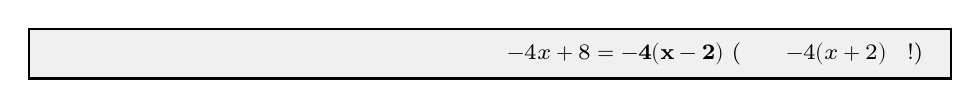
\begin{tikzpicture}
    \node[draw=black, line width=0.8pt, fill=panelgray, inner xsep=10pt, inner ysep=5pt, font=\footnotesize] {ប្រយ័ត្នសញ្ញាដក៖ ពេលចាប់សញ្ញាដកនៅមុខវង់ក្រចក ត្រូវប្ដូរសញ្ញាតួខាងក្នុង៖ $-4x + 8 = \mathbf{-4(x - 2)}$ (មិនមែន $-4(x+2)$ ទេ!)};
  \end{tikzpicture}\par}
\end{tcolorbox}

\newpage
% ============================================================================
% ទំព័រទី២៖ E4 (លំហាត់គំរូ C, D + ១៥, ១៦ ទំ.៧៤) + E5 (ប្រតិបត្តិ + Exit Check) + កិច្ចការផ្ទះ
% ============================================================================

% -------------------- ផ្នែកទី៤៖ E4 ELABORATE --------------------
\secbar{ផ្នែកទី៤ ៖ អនុវត្តលំហាត់គំរូ និងប្រៀបធៀបយុទ្ធសាស្ត្រ \enbf{(E4 — Elaborate)}}{\en{10} នាទី (បំពេញតាមគំរូ)}

\textbf{១. លំហាត់គំរូ $C, D$ (ទំ.៧១--៧២) និងលំហាត់បំពេញការេទី ១៦ ក--ខ (ទំ.៧៤)៖}
\begin{itemize}[leftmargin=0.5cm, itemsep=4.5pt, topsep=2pt]
  \item \textbf{គំរូ $C$ (ទំ.៧២)៖} $C = (a - 4)(y + 2) - (a - 4)(3y + 2) = (a - 4)(y + 2 - 3y - \dotline{0.7cm}) = \dotline{3.2cm}$ ។
  \item \textbf{គំរូ $D$ (ទំ.៧២ — កត្តារួម + ផលបូកពីរគូប)៖} $D = x^3(x + 1) + y^3(x + 1) = (x + 1)(x^3 + y^3) = \dotline{4.8cm}$ ។
  \item \textbf{លំហាត់ទី១៦ ក--ខ (ទំ.៧៤)៖} គេឱ្យ $A = b^2 + 8b + 15$ ។ ត្រូវថែមចំនួន $\dotline{1.0cm}$ លើ $b^2+8b$ ដើម្បីបានការេទ្វេធា $(b + \dotline{0.8cm})^2$ ។\\
  ដូចនេះ $A = (b^2 + 8b + 16) - 16 + 15 = (b + 4)^2 - 1^2 = (\dotline{2.0cm})(\dotline{2.0cm})$ ។
  \item \textbf{ផលដកពីរការេនៃកញ្ចប់ (១៣ឋ ទំ.៧៤)៖} $9a^2 - (a + 2)^2 = [3a - (a+2)][3a + (a+2)] = (2a-2)(4a+2) = \dotline{3.0cm}$ ។
\end{itemize}

\vspace{4.5pt}
\textbf{២. អនុវត្តបំបែកតួកណ្ដាលលើត្រីធា $ax^2 + bx + c$ (លំហាត់ទី១៥ ក, ខ, ង ទំ.៧៤)៖}
\begin{itemize}[leftmargin=0.5cm, itemsep=4.5pt, topsep=2pt]
  \item \textbf{១៥ក ($a=1$)៖} $x^2 + 3x + 2 = x^2 + x + 2x + 2 = \dotline{3.8cm}$ \quad (ព្រោះ $1\times 2 = 2$ និង $1 + 2 = 3$) ។
  \item \textbf{១៥ខ ($a=3, c=8 \implies ac=24$)៖} $3x^2 + 14x + 8 = 3x^2 + \dotline{1.2cm} + \dotline{1.2cm} + 8 = (\dotline{2.0cm})(\dotline{2.0cm})$ ។
  \item \textbf{១៥ង (ចាប់កត្តារួម $2$ សិន)៖} $14a^2 + 18a - 20 = 2(7a^2 + 9a - 10) = 2(7a^2 + 14a - 5a - 10) = \dotline{3.8cm}$ ។
  \item \textbf{ឆ្លុះបញ្ចាំង (\en{Looking Back})៖} ដើម្បីផ្ទៀងផ្ទាត់ថាការដាក់កត្តាត្រឹមត្រូវ ១០០\% យើងគ្រាន់តែគុណតួមុខ និងតួចុងក្នុងចិត្តមើល!
\end{itemize}

% -------------------- ផ្នែកទី៥៖ E5 EVALUATE --------------------
\secbar{ផ្នែកទី៥ ៖ ហ្វឹកហាត់សំយោគចុងមេរៀនទី៥ និងតេស្តរហ័ស \enbf{(E5 — Evaluate)}}{\en{10} នាទី (ធ្វើដោយខ្លួនឯង រួចប្ដូរផ្ទៀង)}

\textbf{១. ចូរដាក់កន្សោមខាងក្រោមជាផលគុណកត្តា (សៀវភៅគោល ទំ.៧៤ — លំហាត់ទី១២, ១៥ និង ១៦គ)៖}

\vspace{2pt}
{\renewcommand{\arraystretch}{1.52}
\begin{tabular}{|L{9.1cm}|L{9.1cm}|}
\hline
\cellcolor{headgray}\textbf{១) ត្រីធា — បំពេញការេ ឬបំបែកតួកណ្ដាល (ទំ.៧៤)} & \cellcolor{headgray}\textbf{២) ការផ្ដុំតួ និងកញ្ចប់កត្តារួម (ទំ.៧៤)} \\
\hline
ក. $B = x^2 + 4x + 3 = \dotline{4.5cm}$ & ក. $8ax - bx + 8ay - by = \dotline{4.0cm}$ \\
\hline
ខ. $C = 4x^2 - 8x + 3 = \dotline{4.4cm}$ & ខ. $ax + ay - 2bx - 2by = \dotline{4.0cm}$ \\
\hline
គ. $2x^2 + 15x + 7 = \dotline{4.8cm}$ & គ. $(2x-3)(5x-1) - (2x-3)(x+1) = \dotline{2.5cm}$ \\
\hline
ឃ. $6x^2 + 5x + 1 = \dotline{4.9cm}$ & ឃ. $x^2 - 6x + 9 - y^2 = \dotline{4.5cm}$ \\
\hline
ង. $x^2 - 6x + 8 = \dotline{4.9cm}$ & ង. $x^3 + 3x^2 - x - 3 = \dotline{4.4cm}$ \\
\hline
\cellcolor{panelgray}ពិនិត្យ៖ $x^2 + 2x - 15 = \dotline{4.3cm}$ & \cellcolor{panelgray}ពិនិត្យ៖ $(a-1)^2 - 9 = \dotline{4.5cm}$ \\
\hline
\end{tabular}}

\vspace{4pt}
\begin{tcolorbox}[enhanced, sharp corners, colback=panelgray, colframe=black, boxrule=0.85pt, top=3pt, bottom=3pt, left=6pt, right=6pt]
  \textbf{២. បិទបេសកកម្ម \en{E1} និងតេស្តរហ័ស (\en{Exit Check — 60} វិនាទី)៖}\\[2pt]
  $\bullet$ \textbf{ចម្លើយបេសកកម្ម \en{E1}៖} $x^2 - 2x - 8 = (x - 1)^2 - 3^2 = \dotline{3.5cm}$ ។\\[2pt]
  $\bullet$ \textbf{សំណួរតេស្តរហ័ស៖} តើត្រីធា $x^2 - 4x - 5$ ដាក់ជាផលគុណកត្តាស្មើនឹងជម្រើសណា? (គូសរង្វង់ជម្រើសត្រឹមត្រូវ)\\[1.5pt]
  \hspace*{0.3cm}\enbf{A.}\; $(x - 5)(x - 1)$ \qquad\quad
  \enbf{B.}\; $(x + 5)(x - 1)$ \qquad\quad
  \enbf{C.}\; $(x - 5)(x + 1)$ \qquad\quad
  \enbf{D.}\; $(x - 2)^2 - 5$
\end{tcolorbox}

% -------------------- ផ្នែកទី៦៖ កិច្ចការផ្ទះ --------------------
\secbar{ផ្នែកទី៦ ៖ ប័ណ្ណកិច្ចការផ្ទះ \enbf{(Homework)} និងការអានមេរៀនថ្មីជាមុន}{សៀវភៅសិក្សាគោល ទំ.៧៣--៧៦}

\begin{tcolorbox}[enhanced, sharp corners, colback=white, colframe=black, boxrule=0.8pt, borderline={0.6pt}{2pt}{dashed}, top=3pt, bottom=3pt, left=6pt, right=6pt]
  \textbf{១. លំហាត់ទី១១ ច (ទំ.៧៣)៖} ដាក់ជាផលគុណកត្តា $(2a - 2b + 10) + (a - b)(a - b + 5)$ \textit{(ចាប់ $2$ ពី $2a-2b+10$ សិន!)} ។\\[1.5pt]
  \textbf{២. លំហាត់ទី១២ (ខ, គ, ង) ទំ.៧៤៖} ខ) $(7a-1)^2 - (7a-1)(3a+2)$ \;;\; គ) $(2x+3)^2 - (2x+3)(5x-7)$ \;;\; ង) $(y-8)(4y-1) + y^2 - 8y$ ។\\[1.5pt]
  \textbf{៣. លំហាត់ទី១៥ ញ (ទំ.៧៤)៖} ដាក់ជាផលគុណកត្តា $14x^2 + 32x + 8$ ។\\[1.5pt]
  $\bullet$ \textbf{អានជាមុន៖} \textbf{មេរៀនទី៦ កន្សោមសនិទាន} — ចំណុចទី១ និងទី២ \textbf{សញ្ញាណ និងតម្លៃលេខនៃកន្សោមសនិទាន} (ទំព័រ ៧៥--៧៦) ។
\end{tcolorbox}

\end{document}
